
\begin{figure}[htbp]
    \centering
    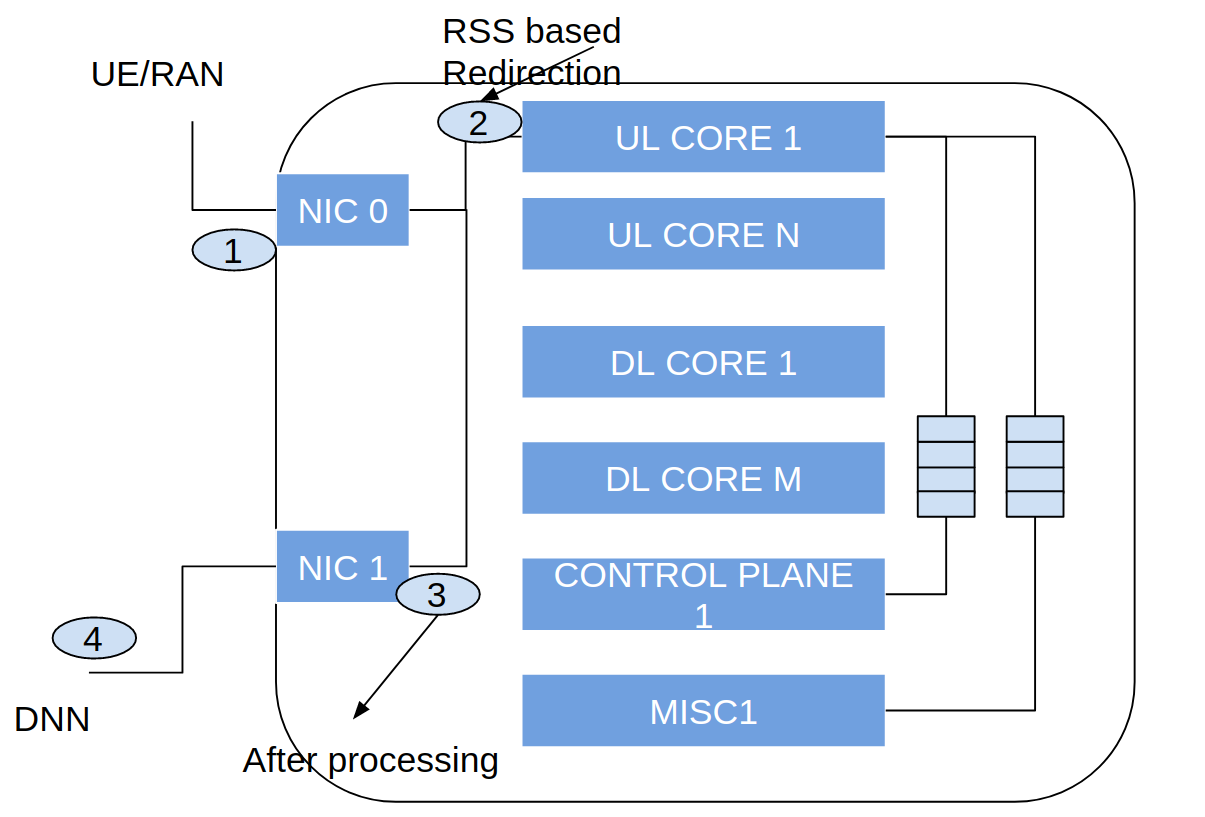
\includegraphics[width=0.9\textwidth, keepaspectratio]{./fig/Introduction/UPF2.png}
    \caption{UPF Architecture}
    \label{figUPF}
\end{figure}
\begin{itemize}
        \item \textbf{Connections} The UPF server is connected to Radio Access Network (RAN) on Port 0 
        and to the Internet through Data Network Name (DNN) on Port 1.
        \item \textbf{Uplink Cores}  Uplink cores are the cores dedicated for handling uplink traffic.
        \item \textbf{Downlink Cores}         Downlink cores are the cores dedicated for handling downlink traffic.
        \item \textbf{Control Plane Core} This core handles the session establishment messages coming from the 
        Session Management Function (SMF). These messages arrive on port 0 and are redirected to uplink cores. 
        Uplink core transfer these messages to control plane core through a circular queue.
        \item \textbf{Miscellaneous Core} This core is responsible for sending heartbeat messages and for handling ARP requests for MAC address (as raw packets are received in  user space and no kernel-level functions available).
\end{itemize}
Figure \ref{figUPF} shows the UPF architecture and packet flow in uplink direction. 